\chapter{Entregable 2}

\begin{itemize}
	\item El preprocesamiento es uno de los procesos más importantes en el flujo de acciones sobre un conjunto de datos. Es determinante para la obtención de modelos con buen rendimiento.
	\item Cada conjunto de datos necesita un preprocesamiento concreto diferente del realizado a otros.
\end{itemize}

\section{Preprocesamiento conjunto de datos de altura de ola}

Describa las operaciones de procesamiento que ha realizado sobre la base de datos proporcionada y como queda la base de datos al final ya procesada.

\subsection{Atributos TIDE, VIS, MWD}
Eliminaremos aquellos atributos que tengan más del 40\% de datos perdidos.
Como podemos comprobar los atributos TIDE, VIS, MWD no aportan nada a nuestro modelo, ya que todos sus valores son nulos. Eliminaremos estos tres atributos de la base de datos, quedándonos con los 15 restantes. Podemos utilizar el filtro Remove explicado en el capitulo anterior. (\ref{fig:filtro_remove})

%En nuestro caso no es necesario cambiar los atributos nominales a binarios, puesto que todos son numericos. 

El atributo DEWP tiene 33\% de los valores perdidos (\ref{fig:DEWP_missing}), por lo tanto también hemos decidido eliminarlo, pues tendríamos que reemplazar todos esos valores por la media e insertaríamos muchos datos iguales en la base de datos.

\begin{figure}[H]
	\centering
	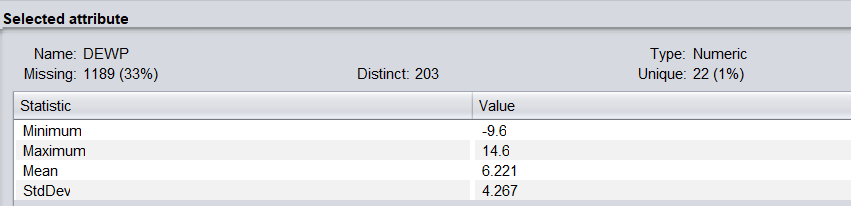
\includegraphics[width=\textwidth, height=0.35\textwidth]{DEWP_missing}
    \caption{DEWP Datos perdidos}
    \label{fig:DEWP_missing}
\end{figure}

\subsection{Recuperación de datos perdidos}

Existen muchas técnicas para la recuperación de datos perdidos.
\begin{itemize}
	\item Reemplazar por la media del conjunto de datos. También se puede reemplazar por la mediana o la moda dependiendo del tipo de atributo. Es un poco más justa cuando se emplean patrones de la misma clase.
	\item Regresión entre atributos (sin datos perdidos).
	\item Mediante técnicas de Machine Learning.
\end{itemize}
\newpage

\begin{wrapfigure}{l}{0.36\textwidth}
	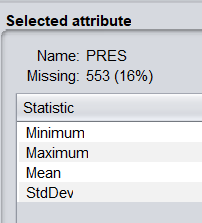
\includegraphics[width=0.9\linewidth, height=5cm]{PRES_1}
	\caption{Atributo PRES}
	\label{fig:PRES}
\end{wrapfigure}

El atributo PRES tiene el 16\% de datos perdidos (Fig\ref{fig:PRES}). 
En nuestro caso hemos utilizado el reemplazo por la media, para hacer esto utilizamos el filtro ``ReplaceMissingValues'' explicado en el capítulo anterior, (Fig\ref{fig:ReplaceMissingValues}) este filtro no calcula la media dependiendo del atributo clase si no que le asigna la misma media a todos. Al utilizar el filtro veremos como el porcentaje ``Missing'' se pone a 0\%.

\subsection{Selección de atributos}

Consiste en obtener una representación reducida del conjunto de datos que preserve información importante de la base de datos. Objetivos: 

\begin{itemize}
	\item Reducir la complejidad del problema eliminando atributos irrelevantes o redundantes.
	\item Aumentar el rendimiento de los modelos.
	\item Acelerar el proceso de aprendizaje.
	\item Reducción del sobreajuste.
\end{itemize}

Aunque en Weka hay muchas formas de seleccionar atributos (como análisis de correlaciones), nos centraremos en el método mediante búsqueda + evaluación. Seleccionamos como: $ ``Attribute evaluator'' \rightarrow CfsSubsetEval$ y como $ ``Search Method'' \rightarrow BestFirst $  
En la (Figura\ref{fig:Seleccion_atributos}) comprobamos como nos selecciona los atributos 2,4,5,7,8,9,10,11,12.

\begin{figure}[H]
	\centering
	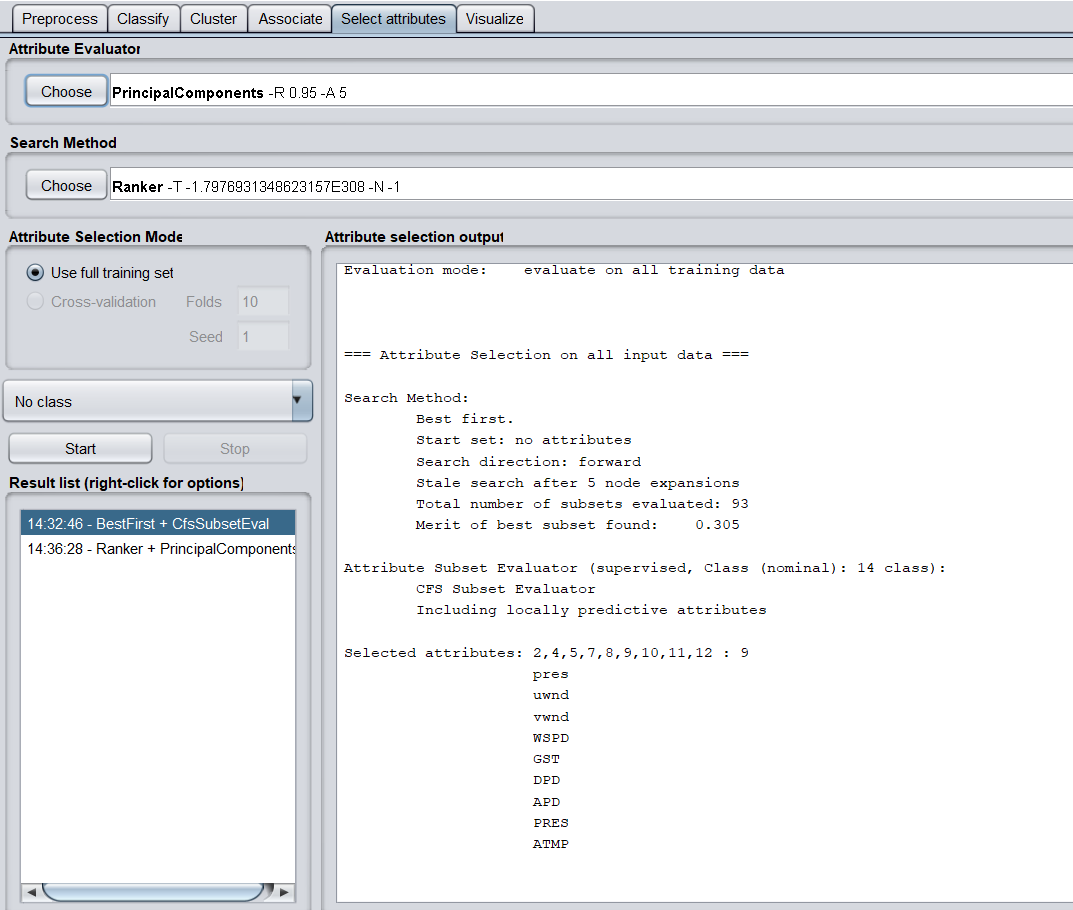
\includegraphics[width=\textwidth, height=\textwidth]{Seleccion_atributos}
    \caption{Seleccion de atributos}
    \label{fig:Seleccion_atributos}
\end{figure}

Volviendo a nuestro conjunto de entrenamiento procedemos a utilizar el filtro ``Remove'' para dejar solo los atributos indicados, para ellos copiamos y pegamos los atributos e invertimos la selección para que nos elimine los no seleccionados (en este caso eliminaremos los atributos AIR, RHUM, WDIR, WTMP). Una vez tenemos los atributos procedemos a realizar un experimento con un clasificador ``Logistic'' y la configuración por defecto para comprobar si hemos mejorado el rendimiento y los atributos eliminados no aportaban mucha información. (\ref{fig:Logistic_rendimiento})

\begin{figure}[H]
	\begin{subfigure}[H]{\textwidth}
    	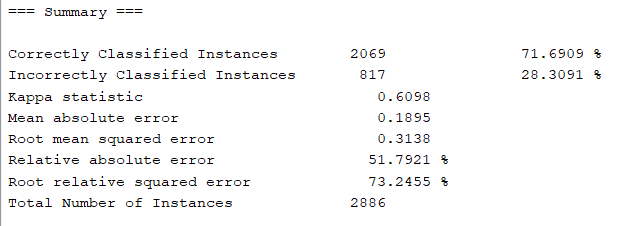
\includegraphics[width=\linewidth]{logistic_1}	
    	\caption{Antes}
	\end{subfigure}
	\hfill
	\begin{subfigure}[H]{\textwidth}
    	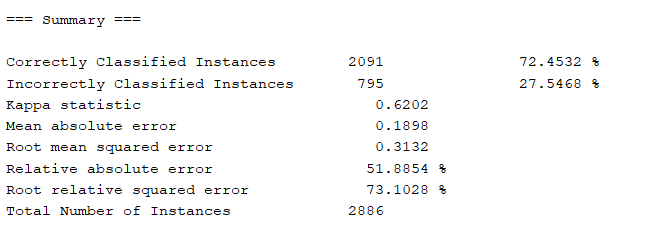
\includegraphics[width=\linewidth]{logistic_select}	
    	\caption{Despues}
   
	\end{subfigure}
	\caption{Logistic rendimiento}
	\label{fig:Logistic_rendimiento}
\end{figure}

\subsection{Correlación}

El rendimiento de algunos algoritmos puede deteriorarse si dos o más variables están estrechamente relacionadas. Eliminar algunas de las variables pueden mejorar el rendimiento del modelo.
Para obtener la matriz de correlaciones nos situamos en la pestaña de selección de atributos y seleccionamos como: $ ``Attribute evaluator'' \rightarrow PrincipalComponents$ y como $ ``Search Method'' \rightarrow Ranked $

\begin{table}[H]
	\resizebox{1.07\textwidth}{!}{
	\begin{tabular}{|l|c|c|c|c|c|c|c|c|c|}
	\hline
	& pres & uwnd & vwnd & WSPD & GST & DPD & APD & PRES & ATMP \\ \hline
	pres & 1 & 0.14 & -0.2 & -0.34 & -0.37 & -0.26 & -0.43 & 0.93 & 0.26 \\
	uwnd & 0.14 & 1 & -0.17 & -0.07 & -0.17 & -0 & -0.03 & 0.05 & 0.17 \\
	vwnd & -0.2 & -0.17 & 1 & 0.31 & 0.31 & 0.07 & 0.13 & -0.18 & -0.01 \\
	WSPD & -0.34 & -0.07 & 0.31 & 1 & \color{red}0.99 & 0.01 & 0.1 & -0.31 & -0.17 \\
	GST & -0.37 & -0.07 & 0.31 & 0.99 & 1 & 0.04 & 0.14 & -0.34 & -0.2 \\ 
	DPD & -0.26 & -0 & 0.07 & 0.01 & 0.04 & 1 & 0.71 & -0.27 & -0.33  \\
	APD & -0.43 & -0.03 & 0.13 & 0.1 & 0.14 & 0.71 & 1 & -0.44 & -0.44 \\
	PRES & 0.93 & 0.05 & -0.18 & -0.31 & -0.34 & -0.27 & -0.44 & 1 & 0.28 \\
	ATMP & 0.26 & 0.17 & -0.01 & -0.17 & -0.2 & -0.33 & -0.44 & 0.28 & 1\\
	\hline
	\end{tabular}
	}
	\caption{Matriz de correlación}
	\label{tabla:Matrizcorrelacion}
\end{table}

Comprobando la matriz de correlación (Tabla\ref{tabla:Matrizcorrelacion} nos damos cuenta como existe una relación entre el atributo GST y WSPD. Mirando el resto de los atributos hemos decidido eliminar el atributo WSPD, debemos tener cuidado porque este análisis puede llevar a ilusiones o relaciones falsas. Eliminaremos el atributo y haremos algunas pruebas con el conjunto de test en el cual también debemos eliminar los mismos atributos que en el conjunto de entrenamiento (Mirar el siguiente punto relacionado con el conjunto de test). Al realizar las pruebas obtenemos un 72,35\% de acierto en clasificación, anteriormente obtuvimos un 72,45\%, aunque hemos perdido 0,1 es señal de que las variable están relacionadas y no aportan mucho al conjunto de datos. Continuando con este procedimiento y obteniendo otra vez la matriz de correlaciones podemos continuar eliminando algunos atributos más. En nuestro caso hemos eliminado: 
\begin{itemize}
	\item WSPD
	\item PRES
	\item uwnd
\end{itemize} 

\section{Preprocesamiento conjunto Test}

El proceso de procesamiento del conjunto test es prácticamente similar al del conjunto de entrenamiento, con algunas pequeñas diferencias, variando únicamente el proceso de normalización de atributos y el reemplazamiento de los atributos perdidos.

\subsection{Tratamiento de atributos}
Todos los atributos eliminados en el conjunto de datos de entrenamiento deben ser eliminados también en el conjunto de test, tanto los eliminados al principio como los eliminados en el proceso de selección de atributos. También hay que reemplazar los datos perdidos como hicimos con el atributo PRES por ejemplo, este reemplazamiento debe ser por los valores usados en train (podemos hacer uso del filtro ``ReplaceMissingWithUserConstant'').

\subsection{Normalización}
%En nuestro caso no hemos normalizado, pero si fuera necesario.
Para normalizar los datos del conjunto de test debemos obtener todos los mínimos y máximos de cada atributo que podemos ver pinchando encima de cada uno o en el botón de Edit. Una vez tengamos todos los valores debemos utilizar el filtro ``MathExpression''.
En expresión debemos introducir los mínimos y máximos tal como aparece en \ref{fig:Normalizacion}, en ``ignoreRange'' se indicará el índice del atributo, y en ``invertSelection'' lo seleccionaremos en true para que solo realice la normalización del atributo indicado. Este proceso debe realizarse para cada unos de los atributos, indicando para cada uno sus correspondientes valores mínimos y máximos.

\begin{figure}[H]
	\centering
	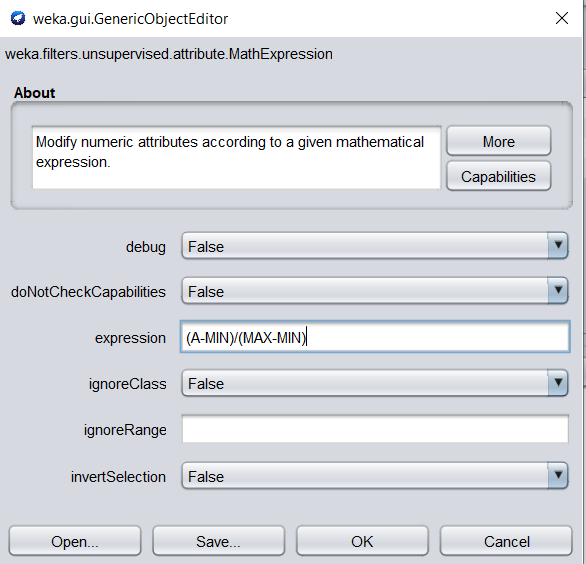
\includegraphics[width=\textwidth]{normalizacion}
    \caption{Filtro Normalizacion}
    \label{fig:Normalizacion}
\end{figure}





